%%%%%%%%%%%%%%%%%%%%%%
\section{Introduction}
%%%%%%%%%%%%%%%%%%%%%%

\begin{frame}[t]\vspace{-1em}
    \titlepage
\end{frame}
\note{
    Welcome to the Sonata and CHERIoT part of this workshop.
    My name is Marno van der Maas and I'm here with Douglas Reis and John Thomson from lowRISC.
}

\begin{frame}
  \frametitle{Morello vs CHERIoT}
  \centering
  \begin{center}
  \begin{tabular}{c c c}
    Address size & 64-bits & 32-bits \\ \hline
    Virtual memory & Yes & No \\ \hline
    Operating system & CheriBSD & CHERIoT RTOS \\ \hline
    RAM size & $>1$ GiB & $<1$ MiB \\
  \end{tabular}
  \end{center}
\end{frame}
\note{
  This morning we were focussed on Morello, how does that exercise compare to the one we will do now?
}

\begin{frame}
    \frametitle{Sonata board}
    \centering
    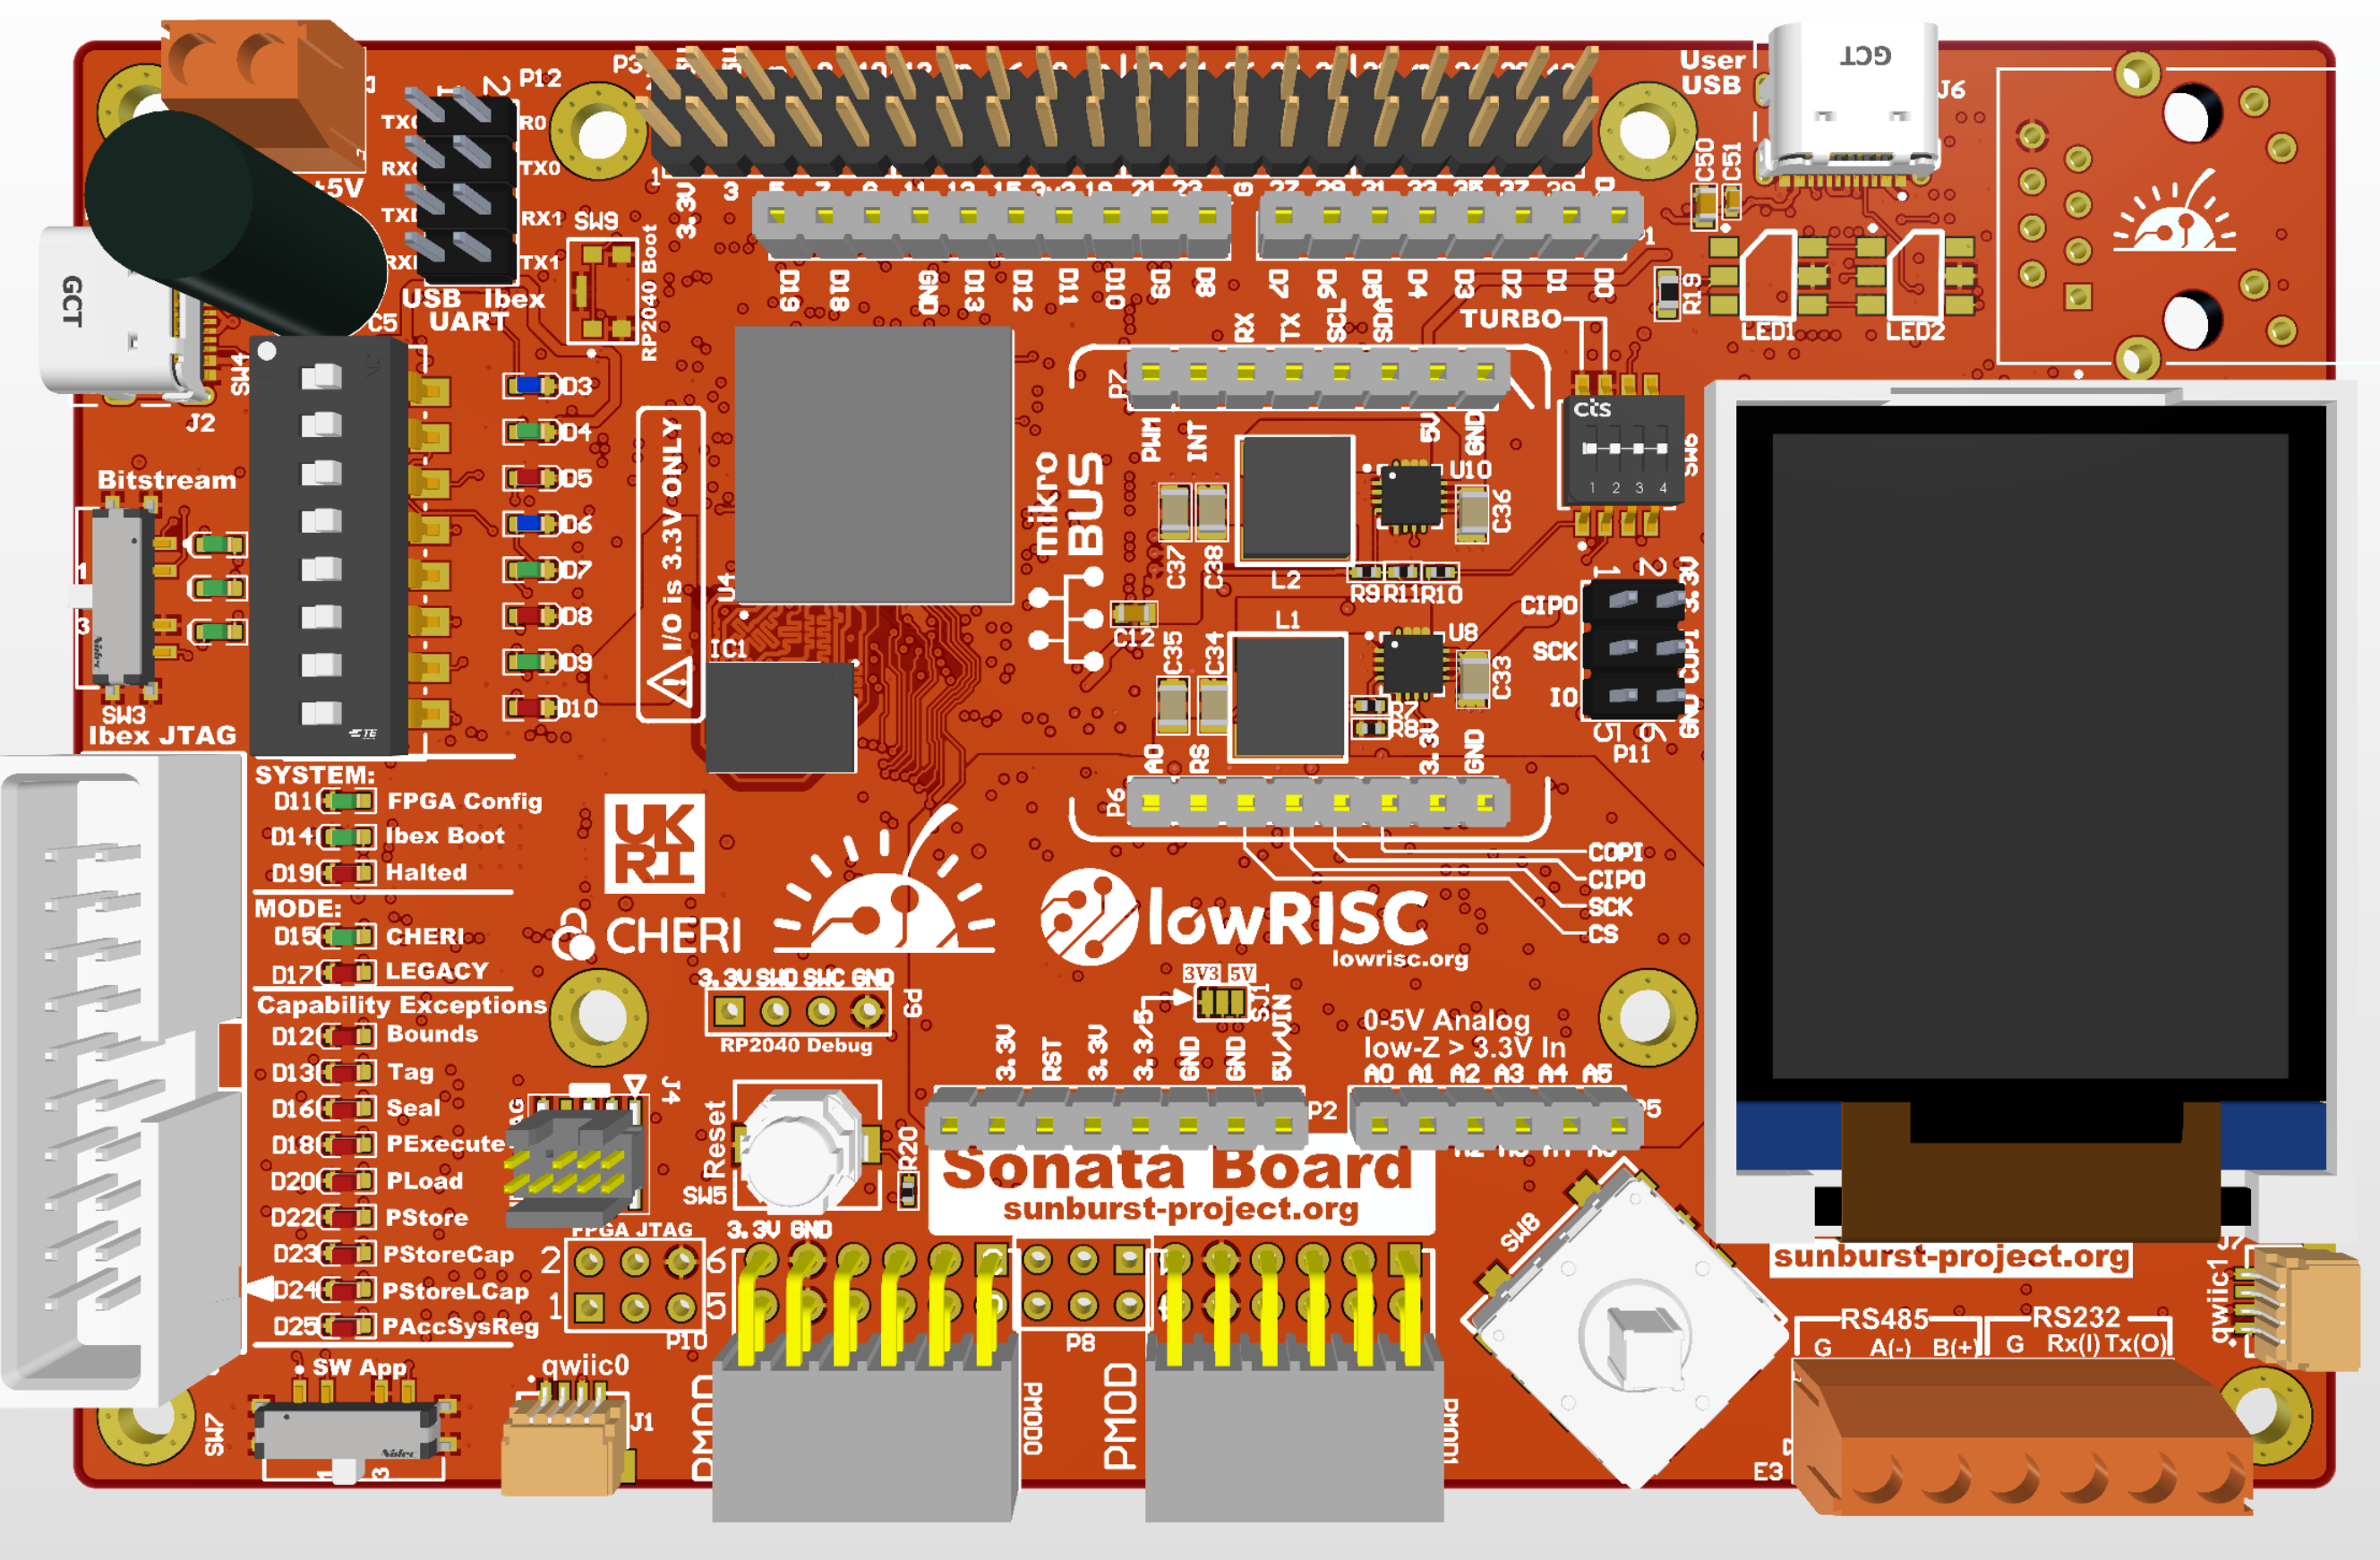
\includegraphics[width=0.7\textwidth]{img/pcb.png}
\end{frame}
\note{
    Here's a picture of an initial version of the Sonata board!
    It is a fully open source platform to get CHERI hardware in the hands of embedded systems engineers.
    Sonata is easy to use, for example USB provides power, allows programming the FPGA and can be used as a serial UART terminal.
}

\begin{frame}
    \frametitle{Why embedded?}
    \centering
    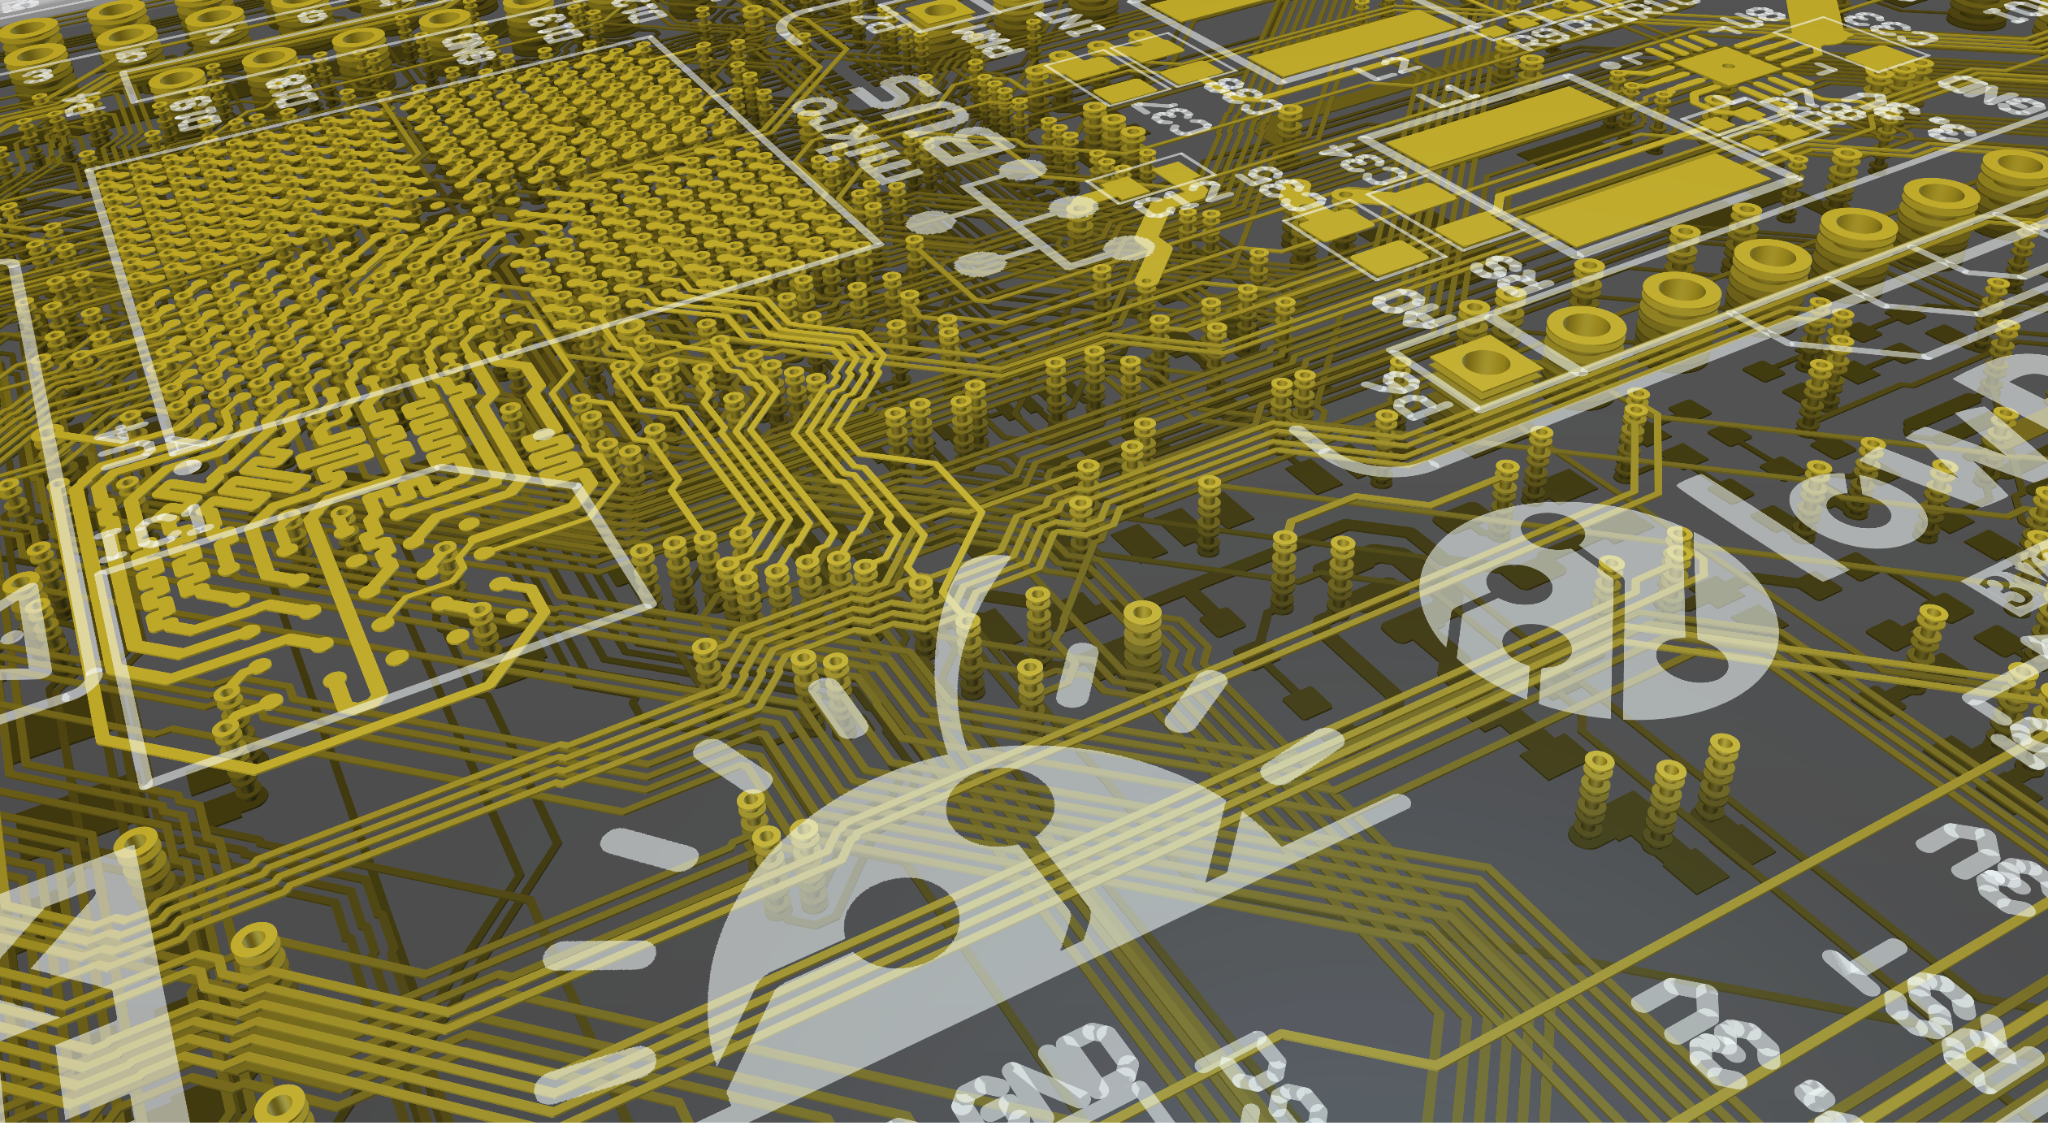
\includegraphics[height=0.7\textheight]{img/embedded.png}
\end{frame}
\note{
    A lot of the initial CHERI research was done on application class processors and proving that the technology could work with rich operating systems, third party applications, a large codebase and modern compilers.
    This was important to prove the technology.

    We believe in the step towards commercialization, embedded systems may be a better place to start because vendors usually have more control over the whole software stack and can recompile everything to use pure capability.
    Sonata can provide the open source platform to make this happen.
}

%%%%%%%%%%%%%%%%%%%%
\section{Background}
%%%%%%%%%%%%%%%%%%%%

\begin{frame}
    \frametitle{Compartentalization}

    \begin{itemize}
        \item Memory allocator
        \item Scheduler
        \item Revoker
    \end{itemize}
\end{frame}
\note{
    CHERIoT puts a lot of emphasis on compartmentatlization to the extent that even a real-time operating system can be compartmentalized in a light-weiht manner.
    \url{https://github.com/search?q=repo\%3Amicrosoft\%2Fcheriot-rtos\%20\_\_cheri\_compartment&type=code}
}

%%%%%%%%%%%%%%%%%%%%%
\section{Design overview}
%%%%%%%%%%%%%%%%%%%%%
\begin{frame}
    \frametitle{Sonata block diagram}
    \centering
    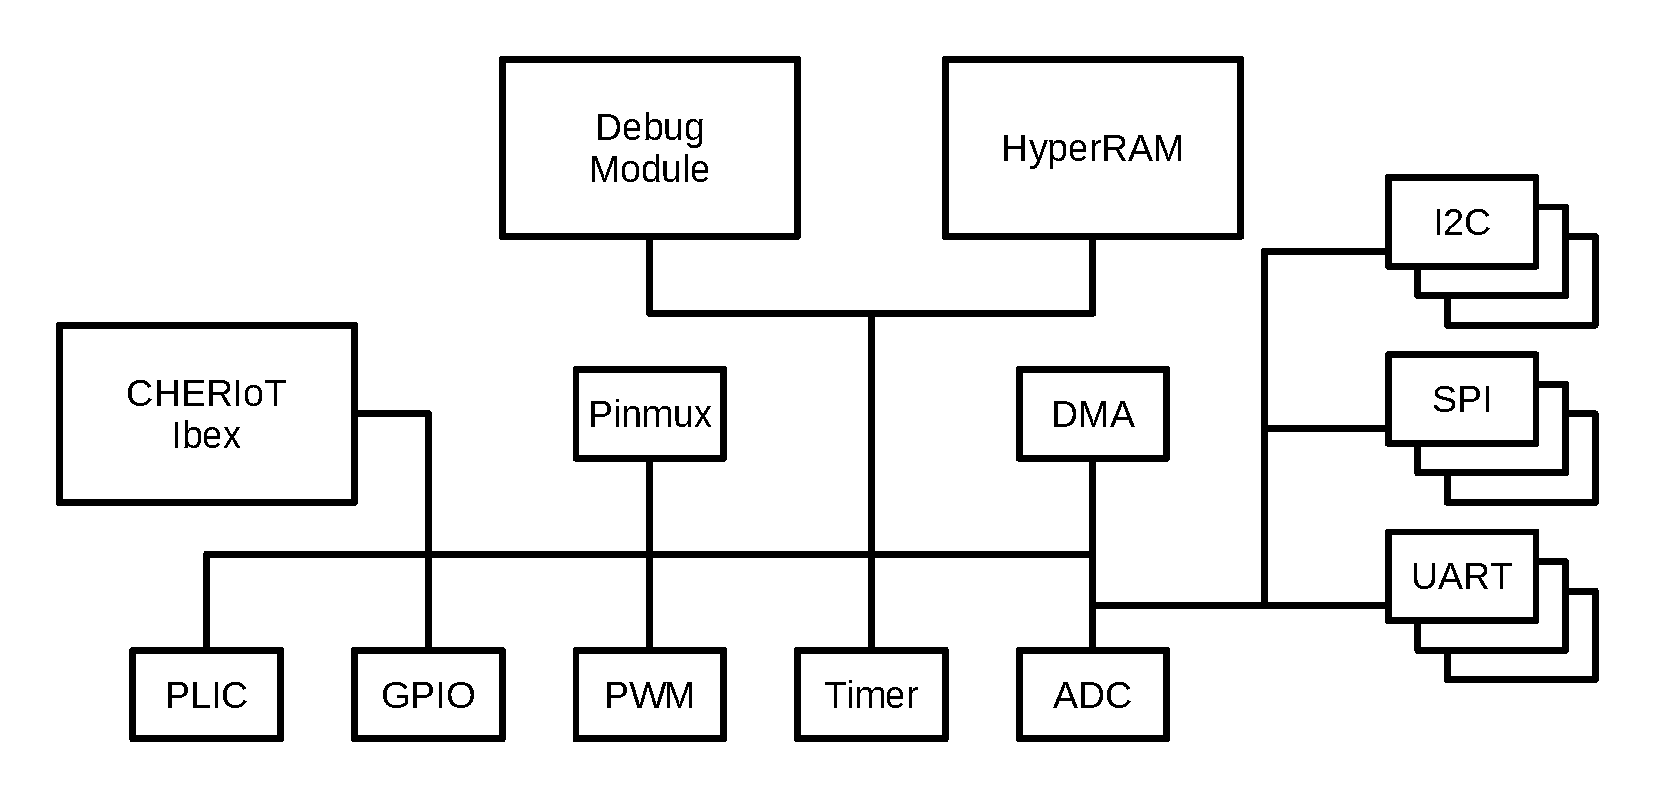
\includegraphics[width=0.9\textwidth]{img/block-diagram.pdf}
\end{frame}
\note{
    Sonata is all about being usable, debuggable, connectable, extendable and interactive.
    To achieve all of this, we need a balance of IP blocks which you can see in this block diagram.

    There is also a big focus on configurability.
    For example the pinmux can be used to drive an LED by a PWM instead of a GPIO.
    And the number of I2C, SPI and UART devices is configurable.
}

\begin{frame}
    \frametitle{Connectable}
    \begin{itemize}
        \item I2C
        \item SPI
        \item UART
        \item GPIO
    \end{itemize}
\end{frame}
\note{
    We support many standard interfaces to connect embedded systems.
    It is important for Sonata, as a development board, to be connectable to as many systems as possible.

    \begin{itemize}
        \item I2C: inter-integrated circuit
        \item SPI: serial peripheral interface
        \item UART: universal asynchronous receiver and transmitter
        \item GPIO: general purpose input and output
    \end{itemize}
}

\begin{frame}
    \frametitle{Extendable}
    \begin{itemize}
        \item Raspberry Pi Hat
        \item Arduino Shield
        \item mikroBus Click
        \item SparkFun QWIIC
        \item PMOD
        \item RS-232 RS-485
    \end{itemize}
\end{frame}
\note{
    And any niche use-cases can be achieved using any of the extension headers provided.
    You can buy off the shelf boards to for example add wireless functionality.
    The hat, shield and click have connectors on the top of the board.
    QWIIC uses I2C to daisy chain boards together (two connectors on the side).
    There are two PMOD connectors on the bottom as well as RS-232 and RS-485 connectors.
}

%%%%%%%%%%%%%%%%%%%%%
\section{Open source}
%%%%%%%%%%%%%%%%%%%%%
\begin{frame}
    \frametitle{Open source at the heart}
    \centering
    \begin{columns} \begin{column}{0.2\textwidth}
        \centering
        
\includegraphics[height=0.2\textheight]{img/llvm.png}
        \\ \vspace{2em}
        
\includegraphics[height=0.2\textheight]{img/freebsd.png}
    \end{column} \begin{column}{0.2\textwidth}
        \centering
        \includegraphics[height=0.2\textheight]{img/riscv.pdf}
        \\ \vspace{4em}
        \includegraphics[width=\textwidth]{img/cheri.pdf}
    \end{column} \begin{column}{0.4\textwidth}
        \includegraphics[width=\textwidth]{img/ibex.pdf}
    \end{column} \end{columns}
\end{frame}
\note{
    The CHERI research benefited from open source projects such as FreeBSD and LLVM.
    CHERIoT Ibex exists because of open architecture (RISC-V, CHERI ISAv9 and CHERIoT ISA) and open silicon (Ibex core).

    The fully open nature of Sonata (RTL, DV, Board layout, software etc) will in turn provide many opportunities for others to continue building on this work.
    Open source can work well to drive innovation and Sonata is playing its part in the CHERI story here.

    \begin{itemize}
        \item \url{https://www.cl.cam.ac.uk/techreports/UCAM-CL-TR-987.pdf}
        \item \url{https://www.microsoft.com/en-us/research/publication/cheriot-rethinking-security-for-low-cost-embedded-systems/}
        \item \url{https://github.com/microsoft/cheriot-ibex}
    \end{itemize}
}

\begin{frame}
    \frametitle{Pull it all together}
    \centering
    \includegraphics[width=0.9\textwidth]{img/platform.pdf}
\end{frame}
\note{
    The idea for Sonata is to be the open source platform that can bring all these efforts together.
    This means taking the work done on open standard instruction set architectures, CPU implementations, compilers, operating systems and software to put them together in an open source platform for embedded systems.
}

\begin{frame}
    \frametitle{Open Sonata}
    \begin{itemize}
        \item Digital design (RTL)
        \item Design verification
        \item Documentation
        \item Software
        \item Board layout
    \end{itemize}
\end{frame}
\note{
    lowRISC's motto is "open to the core".
    Therefore everything is open source from the documentation to the RTL design and to the PCB design.
    The PCB is being manufactured by NewAE technologies, which is a company part of the lowRISC family.
    Here are some links:
    \begin{itemize}
        \item \url{https://github.com/lowRISC/sonata-system}
        \item \url{https://github.com/newaetech/sonata-pcb}
        \item \url{https://lowrisc.org/sonata-system/}
    \end{itemize}
}

\begin{frame}
    \frametitle{Schematic}
    \centering
    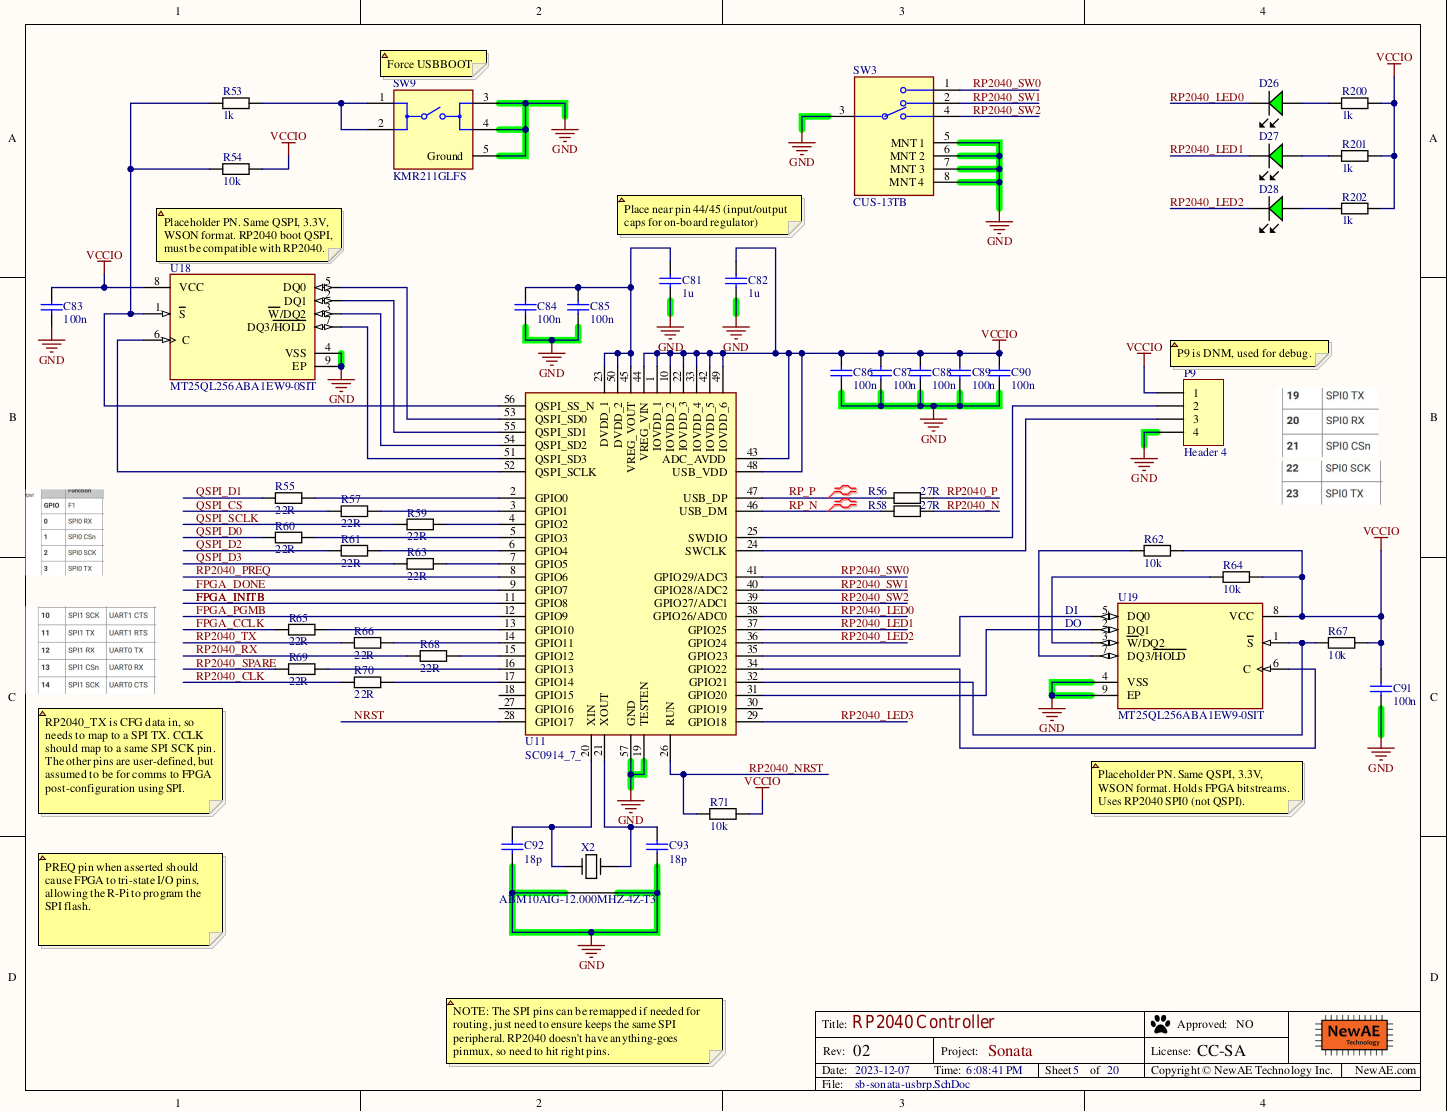
\includegraphics[height=0.8\textheight]{img/schematic.png}
\end{frame}
\note{
    As an example here is part of the PCB schematic published on:
    \url{https://github.com/newaetech/sonata-pcb}
}

